\documentclass[14pt]{beamer}
\usepackage{fancybox}
\usepackage[normalem]{ulem}
%\usepackage{tikz}
%\usepackage{graphicx}

%\centerline{\includegraphics[height=0.5\paperheight]{../Figures/toyMABsimple}}
%\centerline{\includegraphics[width=0.75\paperwidth]{../Figures/joint-partition.pdf}}
%\vspace{-5ex}
% \hyperlink{MCAlgorithm}{\beamergotobutton{Monte Carlo estimation}}

\graphicspath{{Figures/}}

\title{Approximating network reliability\textsuperscript{{\small 1}} \\and Birnbaum importance\textsuperscript{{\small 2}}
}
\date{\\SIAM Workshop on Network Science\\Snowbird\\May 23, 2019}
\author[eubank@virginia.edu]{Stephen Eubank, Madhurima Nath, Yihui Ren\\
\small{NSSAC-TR-19-005}}

\usetheme{CambridgeUS}
\useoutertheme{nssac}
\setbeamertemplate{navigation symbols}{}

\geometry{paperwidth=140mm,paperheight=105mm}
\setbeamercolor{block title}{use=structure,fg=white,bg=black!75!white}
\setbeamercolor{block body}{use=structure,fg=black,bg=black!10!white}

\newenvironment<>{definition}[1]{%
\setbeamercolor{block title}{fg=white,bg=UVABlue}%
\begin{block}#2{Definition: {#1}}}{\end{block}}

\newenvironment<>{remark}[1]{%
\setbeamercolor{block title}{fg=white,bg=UVAOrange}%
\begin{block}#2{Remark: {#1}}}{\end{block}}

\newenvironment<>{example}[1]{%
\setbeamercolor{block title}{fg=white,bg=red!50!blue!50!black!75}%
\begin{block}#2{Example: {#1}}}{\end{block}}

\newenvironment<>{algorithm}[1]{%
\setbeamercolor{block title}{fg=white,bg=blue!50!black}%
\begin{block}#2{Algorithm: {#1}}}{\end{block}}

\setbeamerfont{frametitle}{size=\normalsize}

\DefineNamedColor{named}{darkGreen}{RGB}{147,180,56}
\DefineNamedColor{named}{myPurple}{RGB}{116,24,123}
\DefineNamedColor{named}{myBlue}{RGB}{0,26,245}
\DefineNamedColor{named}{myRed}{RGB}{234,51,35}

%%
%% ----------------------------------------------------------------------
%%
\begin{document}
%%
%% ------------------------------------------------------------------

\begin{frame}
\titlepage

%\vspace{6pt}
\tiny{$^1$E.F.\ Moore and C.E.\ Shannon, Reliable circuits using less reliable relays, Journal of the Franklin Institute, 262, September, 1956.\\
}
\tiny{$^2$Z.W. Birnbaum, in Multivariate Analysis II, Proceedings of the 2nd International Symposium on Multivariate Analysis, ed. by P.R. Krishnaiah (Academic Press, New York, 1969), pp. 581–592}

\end{frame}

%% ----------------------------------------------------------------------

\section{Controlling dynamics on networks}
\subsection{topological control}
\begin{frame}
\frametitle{Why Moore-Shannon reliability and Birnbaum importance matter}
\only<1>{
\centerline{What's the most important edge in a network?}
}
\uncover<2>{
\centerline{\sout{What's the most important edge in a network?}}
\vspace{12pt}
\begin{itemize}
\item \alert{reliability} -- the probability that a dynamical system reaches a configuration with property ${\cal P}$.
\item \alert{Birnbaum importance} -- the contribution of a set of interactions to the reliability.%\\
      %Removing which interaction most reduces the reliability?
%\item Given a budget $B$ and a cost for removing each interaction, which set of interactions should be removed to maximally reduce the reliability?
\end{itemize}
\vspace{12pt}
\centerline{What is the \alert{Birnbaum importance} of
%\begin{itemize}
%\item  
a \alert{set of interactions}}
%\item 
\centerline{with respect to a \alert{property ${\cal P}$}
%\item 
under \alert{dynamics ${\cal D}$}?}
%\end{itemize}
}
\end{frame}


%% ----------------------------------------------------------------------

\begin{frame}
\frametitle{Why do we need to approximate?}
 \centerline{Birnbaum importance is the difference in reliability for 2 networks.}
 \begin{itemize}
\item Evaluating reliability is \alert{\#P-hard}.
\item Interesting instances have $N \sim O(10^{4} - \alert{10^{9}})$ interactions.
\item Birnbaum importance can be \alert{extremely small}, e.g., $2^{-N}$,\\
so Monte Carlo may require exponentially many samples.
\item There are\alert{ $2^N$ possible sets} of interactions to test.
\item Birnbaum importance is \alert{not a submodular} function,\\ 
so greedy algorithms may not work.
\end{itemize}
\end{frame}


%% ----------------------------------------------------------------------

\begin{frame}<1>[label=conclusion]
\frametitle{The thrilling conclusion -- Don't Panic}
For \alert {monotonic properties} ${\cal P}$ under $SIR$ dynamics -- a class which includes cascading failures on layered networks -- Birnbaum importance is well approximated by \alert{Bezier interpolation} between \alert{weak- and strong-coupling approximations} constructed from certain minimal sets of edges (\alert{cruxes}) which can be sampled efficiently using Monte-Carlo. Moreover, Birnbaum importance is a \alert{submodular function} of cruxes, so a greedy approach gives approximations with \alert{bounded errors}.\\
\uncover<2>{
%\vspace{6pt}
\tiny{Nath, M., Ren, Y., Eubank, S., An approach to structural analysis using Moore-Shannon network reliability, in L.M. Aiello et al., Complex Networks 2018, pp. 537-549, 2019\\}
\tiny{Nath, M., Ren, Y., Khorramzadeh, Y., \& Eubank, S. (2018). Determining whether a class of random graphs is consistent with an observed contact network. Journal of Theoretical Biology, 440, 121-132.\\
}
\tiny{
Ren, Y., Eubank, S., \& Nath, M. (2016). From network reliability to the Ising model: A parallel scheme for estimating the joint density of states. Physical Review E, 94(4), 042125.\\
}
\tiny{
Khorramzadeh, Y., Youssef, M., Eubank, S., \& Mowlaei, S. (2015). Analyzing network reliability using structural motifs. Physical Review E, 91(4), 042814.\\ 
}
\tiny{
Eubank, S., Youssef, M., \& Khorramzadeh, Y. (2014). Using the network reliability polynomial to characterize and design networks. Journal of Complex Networks, 2(4), 356-372. doi:10.1093/comnet/cnu037. \\
}
\tiny{
Youssef, M., Khorramzadeh, Y., \& Eubank, S. (2013). Network reliability: The effect of local network structure on diffusive processes. Physical Review E, 88(5), 052810. \\
}
}
\end{frame}

%% ----------------------------------------------------------------------

\section{Formalizing the problem}
\subsection{reliability}
\begin{frame}
\frametitle{Moore-Shannon network reliability}
\begin{definition}{Reliability}
Network reliability $R$ is the probability that the dynamics $D$ on an interaction network $G$ generate a system configuration with property ${\cal P}$:
$$
R \equiv \sum_{c \in \textcolor{red}{\cal C}} \textcolor{blue}{{\cal I_P}}(c) \textcolor{UVAOrange}{p_D}(c) = \langle \textcolor{blue}{{\cal I_P}} \rangle = \sum_{\{c | \textcolor{blue}{{\cal I_P}}(c) = 1\}} \textcolor{UVAOrange}{p_D}(c)
$$
\end{definition}
where 
\begin{itemize}
\item \textcolor{red}{${\cal C}$} is the set of all system configurations; 
\item $\textcolor{blue}{{\cal I_P}}(c)$ indicates whether configuration $c$ has property ${\cal P}$;
\item $\textcolor{UVAOrange}{p_D}(c)$ is the probability that the dynamics generate configuration $c$.
\end{itemize}
\end{frame}

%% ----------------------------------------------------------------------

\begin{frame}
\frametitle{A rose by any other name
}
%\begin{definition}{Reliability}
%Reliability $R$ is the probability that the dynamics $D$ generate a system configuration with property ${\cal P}$:
$$
R \equiv \sum_{c \in {\cal C}} {\cal I_P}(c) p_D(c) = \langle {\cal I_P} \rangle 
$$
%\end{definition}
$R$ is also known as 
\begin{itemize}
\item \alert{Statistical Physics}: a partition function;
\item \alert{Computer Science}: an instance of stochastic satisfiability;
\item \alert{Graph Theory}: an evaluation of the Tutte polynomial.
\item \alert{Engineering}: reliability
\end{itemize}
%\vspace{6pt}
%\centerline{\alert{Reliability depends essentially on $D$ and ${\cal P}$!}}
\end{frame}

%% ----------------------------------------------------------------------

\begin{frame}
\frametitle{Example: Does $S$ infect $T$ under SIR dynamics on $G$?
}
$$
R \equiv \sum_{c \in \textcolor{red}{\cal C}} \textcolor{blue}{{\cal I_P}}(c) \textcolor{UVAOrange}{p_D}(c) = \langle \textcolor{blue}{{\cal I_P}} \rangle = \sum_{\{c | \textcolor{blue}{{\cal I_P}}(c) = 1\}} \textcolor{UVAOrange}{p_D}(c)
$$

\begin{definition}{1-1 mapping between events and edges in $G$}
Event $E_{(i,j)}$ is
an interaction between nodes $i$ and $j$ that leads to $j$ being in the infected state, $I$.
I.e., $E_{(i,j)}\equiv (i$ infects $j$).
\end{definition}
\begin{remark}{Dynamics as subgraph selection}
\begin{itemize}
\item Configuration space \textcolor{red}{${\cal C}$} is the set of all subgraphs of $G$.
\item $\textcolor{blue}{{\cal I_P}}(c)$ is true if and only if $c$ contains a path from $S$ to $T$.
\item $\textcolor{UVAOrange}{p_D}(c)$ is the product of all the transmission probabilities (edge weights) in the subgraph $c$.\\
\end{itemize}
\end{remark}
\end{frame}

%% ----------------------------------------------------------------------

\frame<1-3>[label=BinaryFunc]
{ 
\frametitle{${\cal I_P}$ is a deterministic binary function of $N$ random binary inputs}
\begin{columns}
\begin{column}{0.25\textwidth}
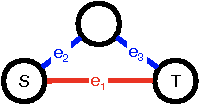
\includegraphics{e1-or-e2-and-e3-base}
\end{column}
\begin{column}{0.75\textwidth}
\only<1-3>{
Configurations that have property ${\cal P}$ (struts):\\
\vspace{10pt}
\begin{tabular}{|c|c|}
\hline
$\textcolor{red}{E_1}\textcolor{blue}{E_2E_3}$ & probability  \\
\hline
\textcolor{red}{T}\textcolor{blue}{TT} &$\textcolor{red}{p_1}\textcolor{blue}{ p_2p_3}$ \\
\textcolor{red}{T}\textcolor{blue}{TF} &$\textcolor{red}{p_1}\textcolor{blue}{ p_2q_3}$ \\
\textcolor{red}{T}\textcolor{blue}{FT} &$\textcolor{red}{p_1}\textcolor{blue}{ q_2p_3}$ \\
\textcolor{red}{T}\textcolor{blue}{FF} &$\textcolor{red}{p_1}\textcolor{blue}{ q_2q_3}$ \\
\textcolor{red}{F}\textcolor{blue}{TT} &$\textcolor{red}{q_1}\textcolor{blue}{ p_2p_3}$ \\
\hline
\end{tabular}
}
\only<1>{
(with 
\begin{tabular}{c}
$q_i \equiv 1 - p_i$\\
$e_ie_j \equiv e_i \land e_j$
\end{tabular}
)
}
\only<2-3>{
%\hfil
\begin{tabular}{|c|c|}
\hline
\textcolor{red}{$E_1$}\textcolor{blue}{$E_2E_3$} & probability\\
\hline
\textcolor{red}{T }\textcolor{blue}{\#\#} & $\textcolor{red}{p_1}$\\
\textcolor{red}{\#}\textcolor{blue}{ TT} & $\textcolor{blue}{ p_2p_3}$\\
\hline
\end{tabular}
}
\only<4>{
%\vspace{18pt}
Configurations that don't have property ${\cal P}$ (cuts):\\
\vspace{10pt}
%\centerline{
\begin{tabular}{|c|c|}
\hline
$\textcolor{red}{E_1}\textcolor{blue}{E_2E_3}$ & probability  \\
\hline
\textcolor{red}{F}\textcolor{blue}{ TF} &$\textcolor{red}{q_1}\textcolor{blue}{ p_2q_3}$\\
\textcolor{red}{F}\textcolor{blue}{ FT} &$\textcolor{red}{q_1}\textcolor{blue}{ q_2p_3}$\\
\textcolor{red}{F}\textcolor{blue}{ FF} &$\textcolor{red}{q_1}\textcolor{blue}{ q_2q_3}$\\
\hline
\end{tabular}
%\hfil
\begin{tabular}{|c|c|}
\hline
$\textcolor{red}{E_1}\textcolor{blue}{E_2E_3}$ & probability  \\
\hline
\textcolor{red}{F}\textcolor{blue}{ F\#} & $\textcolor{red}{q_1}\textcolor{blue}{ q_2}$\\
\textcolor{red}{F}\textcolor{blue}{ \#F} & $\textcolor{red}{q_1}\textcolor{blue}{ q_3}$\\
\hline
\end{tabular}
}
\end{column}
\end{columns}

\vspace{10pt}
SSAT: \phantom{\ \ \ \ }
\only<1>{
$p(
\textcolor{red}{e_1}\textcolor{blue}{e_2e_3}\,  \lor 
\textcolor{red}{e_1}\textcolor{blue}{e_2\overline{e}_3}\,  \lor
\textcolor{red}{e_1}\textcolor{blue}{\overline{e}_2e_3}\,  \lor
\textcolor{red}{e_1}\textcolor{blue}{\overline{e}_2\overline{e}_3}\,  \lor
\textcolor{red}{\overline{e}_1}\textcolor{blue}{e_2e_3}
)
$
}
\only<2-3>{
$p(
\textcolor{red}{e_1} \lor
\textcolor{blue}{e_2e_3}
) \quad \leftarrow$ minimal struts $\in$ cruxes
}
\only<4>{
$p(
\textcolor{red}{\overline{e}_1} \textcolor{blue}{\overline{e}_2}\lor
\textcolor{red}{\overline{e}_1} \textcolor{blue}{\overline{e}_3}
) \quad \leftarrow$ minimal cuts $\in$ cruxes
}

Reliability =
\only<1-3>{
$\textcolor{red}{p_1}\textcolor{blue}{p_2p_3} +
\textcolor{red}{p_1}\textcolor{blue}{p_2q_3} +
\textcolor{red}{p_1}\textcolor{blue}{q_2p_3} +
\textcolor{red}{p_1}\textcolor{blue}{q_2q_3} +
\textcolor{red}{q_1}\textcolor{blue}{p_2p_3}$
}
\only<2>{
\hphantom{Reliability }
$=\textcolor{red}{p_1} + \textcolor{blue}{p_2p_3} 
- \textcolor{red}{p_1}\textcolor{blue}{p_2p_3}$
}
\only<3>{
\hphantom{Reliability }
$=\textcolor{red}{p_1} + \textcolor{blue}{p_2p_3} 
\Ovalbox{$- \textcolor{red}{p_1}\textcolor{blue}{p_2p_3}$}$\\
\vspace{6pt}
Corrects for counting the configuration \textcolor{red}{T}\textcolor{blue}{TT}  twice.
}
\only<4>{
$\textcolor{red}{q_1}\textcolor{blue}{ p_2q_3} +
\textcolor{red}{q_1}\textcolor{blue}{ q_2p_3} +
\textcolor{red}{q_1}\textcolor{blue}{ q_2q_3}$\\
\hphantom{Reliability}
$={\rm \ \ \ }\textcolor{red}{q_1}\textcolor{blue}{ q_2}+\textcolor{red}{q_1}\textcolor{blue}{ q_3} 
- \textcolor{red}{q_1}\textcolor{blue}{ q_2q_3}$\\
\hyperlink{Exploiting}{\beamerreturnbutton{return}}
}
}
%\end{frame}

%% ----------------------------------------------------------------------

\subsection{inclusion-exclusion}
\begin{frame}[label=Taylor]
\frametitle{The inclusion-exclusion expansion corrects for overcounting}
\begin{definition}{The inclusion-exclusion expansion}
$$p(a_1 \lor a_2) = p(a_1) + p(a_2) - p(a_1 \land a_2)$$
\end{definition}
Recursively,\\
$$
p(\bigvee_{i=1}^M a_i) = \sum_{i=1}^M p(a_i) - \sum_{i>j=1}^M p(a_i \land a_j) + \sum_{i>j>k=1}^M p(a_i \land a_j \land a_k) - \cdots
$$
For monotonic properties, this generates a Taylor series.
\hyperlink{monotonicity}{\beamergotobutton{monotonicity}}

\end{frame}

%% ----------------------------------------------------------------------

\begin{frame}[label=generating]
\frametitle{Inclusion-exclusion for monotonic ${\cal P}$ generates a Taylor series}
\vspace{-36pt}
$$
p(\bigvee_{i=1}^M a_i) = \sum_{i=1}^M p(a_i) - \sum_{i>j=1}^M p(a_i \land a_j) + \sum_{i>j>k=1}^M p(a_i \land a_j \land a_k) - \cdots
$$
\begin{example}{$p(a_i) = x$ and $a_i$ is independent of $a_j$}
$$
p(\bigvee_{i=1}^M a_i) =  M x -  {M \choose 2} x^2 + {M \choose 3} x^3 - \cdots %= 1 - (1-x)^M
$$
\end{example}

\end{frame}

%% ----------------------------------------------------------------------

\subsection{Taylor series}
\begin{frame}
\frametitle{Example for S-T reliability under SIR dynamics}
\centerline{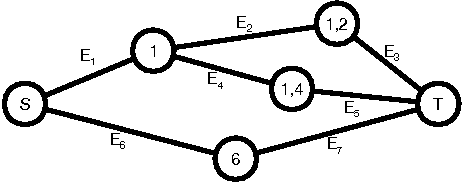
\includegraphics[width=2in]{toySAT.pdf} }
\begin{remark}{a more complicated case}
$a_1$, $a_2$, and $a_3$ are compound events;\\ $a_1$ and $a_2$ are not independent.
\end{remark}
\vspace{-10pt}
\begin{eqnarray*}
R &=& 
%p_D\left((\textcolor{red}{e_1} \land e_2 \land e_3) \lor (\textcolor{red}{e_1} \land e_4 \land e_5) \lor (e_6 \land e_7)\right)\\
%&=& p_D(\textcolor{red}{e_1} \land e_2 \land e_3) + p_D(\textcolor{red}{e_1} \land e_4 \land e_5) + p_D(e_6 \land e_7)\\
% & & \quad - p_D(\textcolor{red}{e_1} \land e_2 \land e_3 \land e_4 \land e_5) - p_D(\textcolor{red}{e_1} \land e_2 \land e_3 \land e_6 \land e_7) - p(\textcolor{red}{e_1} \land e_4 \land e_5 \land e_6 \land e_7)\\
% & & \quad + p_D(\textcolor{red}{e_1} \land e_2 \land e_3 \land e_4 \land e_5 \land e_6 \land e_7)\\
p_D\left((\textcolor{red}{e_1}e_2 e_3) \lor (\textcolor{red}{e_1} e_4 e_5) \lor (e_6 e_7)\right)\\
%&=& p_D(\textcolor{red}{e_1} e_2 e_3) + p_D(\textcolor{red}{e_1} e_4 e_5) + p_D(e_6 e_7)\\
 %& & \quad - p_D(\textcolor{red}{e_1}  e_2 e_3  e_4  e_5) - p_D(\textcolor{red}{e_1} e_2 e_3 e_6  e_7) - p(\textcolor{red}{e_1} e_4 e_5  e_6  e_7)\\
% & & \quad + p_D(\textcolor{red}{e_1}  e_2  e_3 e_4 e_5 e_6 e_7)\\
 &\rightarrow& x^2 + 2x^3 - 3x^5 + x^7
\end{eqnarray*}

Note: $p(\textcolor{red}{e_1}e_2 e_3\textcolor{red}{e_1} e_4 e_5) = p(\textcolor{red}{e_1}e_2 e_3 e_4 e_5) \rightarrow x^5$.
\end{frame}

%% ----------------------------------------------------------------------

\section{Exploiting duality}
\subsection{The dual problem}
\begin{frame}[label=Exploiting]
\frametitle{Reliability has a natural dual}
\vspace{-6pt}
$$
R = \textcolor{UVABlue}{p\left(\bigvee_{i=1}^M a_i\right)} = 1 - p\left(\bigwedge_{i=1}^M \lnot{a}_i\right) = 1 - \textcolor{UVAOrange}{p\left(\bigvee_{j=1}^{\overline{M}} z_j\right)},
$$
\textcolor{UVABlue}{$a_i$ is a conjunction of independent events}\\
$$a_i = \left\{e_{i,1}, e_{i,2},\ldots, e_{i,m_i}\right\};
\quad p(a_i) = \prod_{k=1}^{m_i} \textcolor{UVABlue}{p(e_{i,k})}$$
\textcolor{UVAOrange}{$z_j$ is a conjunction of independent ``anti-events''}\\
$$z_j=\left\{\overline{e}_{j,1}, \overline{e}_{j,2}, \ldots, \overline{e}_{j,\overline{m}_j}\right\}; 
\quad p(z_j) = \prod_{\ell=1}^{\overline{m}_j} \textcolor{UVAOrange}{[1 - p(e_{j,\ell})]}$$

\hyperlink{BinaryFunc<4>}{\beamergotobutton{SSAT}}

\end{frame}

%% ----------------------------------------------------------------------

\subsection{a strong-coupling approximation}
\begin{frame}
\frametitle{The dual generates a strong-coupling expansion}

\begin{remark}{Taylor series as perturbative expansions}
The probability of an interaction between two nodes, $x$, is a coupling constant in the dynamics.
%If $R\colon [0,1] \to [0,1]$ is a finite-degree polynomial in $x$, 
Truncated Taylor series for $R$ at $x=0$ are ``perturbative estimates'' for $R$, known in statistical physics as {\em weak-coupling} expansions. Strong-coupling expansions are truncated Taylor series at the ``other end'' of the domain, here $x=1$.
\end{remark}
\end{frame}

%% ----------------------------------------------------------------------

\subsection{interpolating between approximations}
\begin{frame}[label=interpolation]
\frametitle{
\only<1>{\textcolor{myBlue}{Weak} / \textcolor{myRed}{strong} coupling expansions for $\textcolor{myPurple}{R(x)}$ often diverge}
\only<2>{Bezier approximations smoothly \textcolor{black}{interpolate} with tight \textcolor{darkGreen}{bounds}}
}

\centerline{
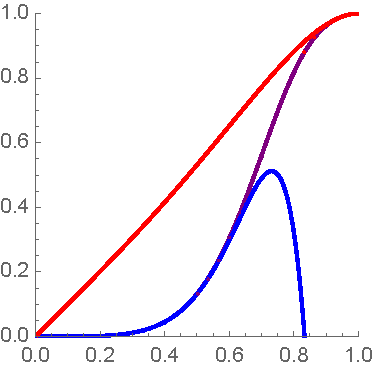
\includegraphics[width=0.45\paperwidth]{../Figures/MathA}
\uncover<2>{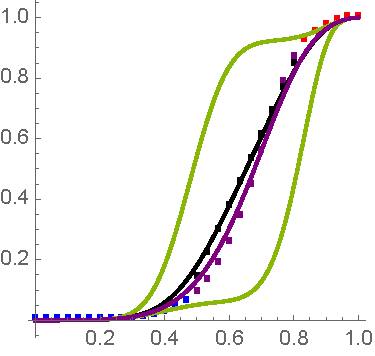
\includegraphics[width=0.45\paperwidth]{../Figures/MathB}}
}
\uncover<2>{
Taylor series are expressed in power bases: $x^k$ or $(1-x)^k$\\
Bezier interpolates in Bernstein basis: $ {N \choose k} x^k (1-x)^{N-k}$\\
\hyperlink{Bezier}{\beamergotobutton{Details}}}

\end{frame}

%% ----------------------------------------------------------------------

\section{Ranking edges}
\subsection{Birnbaum importance}
\begin{frame}
\frametitle{Leave-N-out change in reliability measures influence}
\begin{definition}{Birnbaum importance}
The \alert{Birnbaum importance} of a subset of network elements ${\cal E}$ is the difference in reliability between the network with and without those elements.
$$
B_{{\cal P}} ({\cal G}, {\cal E}) = R_{{\cal P}}({\cal G}) - R_{{\cal P}}({\cal G\setminus{\cal E}})
$$
\end{definition}
\begin{remark}{Birnbaum importance can be tiny}
$\left[R_{{\cal P}}({\cal G}) - R_{{\cal P}}({\cal G\setminus{\cal E}})\right] / R_{{\cal P}}({\cal G})$ can be $O(2^{-N})$.
\end{remark}
\begin{remark}{Greedy approximation is possible}
$B$ is {\em not} submodular in edges, but it {\em is} submodular in cruxes.
\end{remark}
\end{frame}

%% ----------------------------------------------------------------------

\begin{frame}
\frametitle{$R$ is affine in each interaction probability}
$$
p(e_i \land e_i) = p(e_i) \equiv w_i \Longleftrightarrow \frac{\partial R}{\partial w_i} = B(\{e_i\}) / w_i
$$
\begin{remark}{$B$ defines $R$'s sensitivity / tangent plane}
$B$ turns the inherently \alert{discrete} edge ranking problem into a \alert{continuous} gradient descent problem. 
\end{remark}
$$
\frac{\partial R}{\partial w_i} = R|_{w_i=1} - R|_{w_i=0} 
$$
\begin{remark}{Recurrent contraction -- deletion defines Tutte}
$w_i= 1 \rightarrow$ contraction;
$w_i = 0 \rightarrow$ deletion.
\end{remark}

\end{frame}

%% ----------------------------------------------------------------------

\begin{frame}
\frametitle{Improving numerical stability for SIR (and ??) dynamics}

%$$
%B(\{e_1,e_2\}) = \rho_{0,0} + \rho_{1} p(e_1) + \rho_{2} p(e_2) + \rho_{1,2} p(e_1)p(e_2)
%$$

\centerline{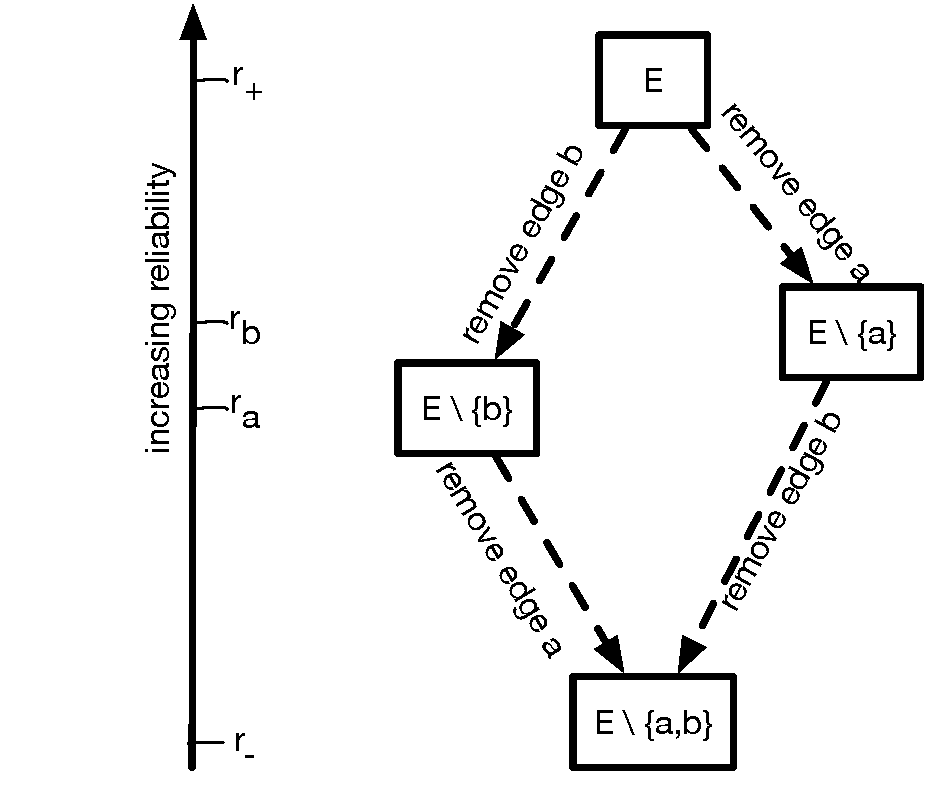
\includegraphics[height=0.5\paperheight]{../Figures/graphReductions}}

\centerline{Evaluate $r_b - r_a$ directly, instead of $r_b$ and $r_a$ separately.}
\end{frame}

%% ----------------------------------------------------------------------

\section{Applications:}
\subsection{overview}
\begin{frame}[label=Applications]
\frametitle{What you can do with these tools}
\begin{itemize}
\item Compare networks \hfill \hyperlink{MCExample}{\beamergotobutton{addHealth}}
\item Define effective couplings \hfill \hyperlink{Renormalization}{\beamergotobutton{renormalization}}
\item Graph reduction minimizing $\Delta R$ \hfill \hyperlink{GraphReduction}{\beamergotobutton{reduction}}
\item Rank edges, find crossover in importance \hfill \hyperlink{CrossoverExample}{\beamergotobutton{crossover}}
\item Find communities in weighted, directed graphs \hfill \hyperlink{Community}{\beamergotobutton{example}}
\item Generate graph duals \hfill \hyperlink{GraphDuals}{\beamergotobutton{duals}}
\end{itemize}
\end{frame}

%% ----------------------------------------------------------------------

\section{}
\subsection{}
\begin{frame}[label=extensions]
\frametitle{(Almost automatic) extensions}
\begin{itemize}
\item Reliability and Birnbaum importance for vertices
\item Reliability and Birnbaum importance on hyper-graphs
\item Other dynamics, especially time-dependent networks
\item Bezier interpolation in the thermodynamic limit ($N \to \infty$)
\item Combine MC and perturbative expansions
\item Find optimal edge weight reductions, not removals 
\item Compare this notion of duality to others
\item Detect graph isomorphisms ??
\end{itemize}
\end{frame}

%% ----------------------------------------------------------------------

\againframe<2>{conclusion}
%\begin{frame}
%\frametitle{Conclusion}
%For \alert {monotonic properties} ${\cal P}$ under $SIR$ dynamics, a class which includes cascading failures, Birnbaum importance is well approximated by \alert{Bezier interpolation} between \alert{weak- and strong-coupling approximations} constructed from certain \alert{minimal sets} of edges (cruxes) which can be sampled efficiently using Monte-Carlo. Moreover, Birnbaum importance is a \alert{submodular function} of these minimal sets, so a greedy approach gives approximations with \alert{bounded errors}.
%\end{frame}

%% ----------------------------------------------------------------------

\appendix

%% ----------------------------------------------------------------------

\section{Formalizing the problem}
\subsection{inclusion-exclusion}
\begin{frame}[label=monotonicity]
\frametitle{Monotonicity, cruxes, cuts, and struts}
\begin{definition}{Monotonicity}
A property is \em{monotonic} if $I_{\cal P}(g) = 1 \Rightarrow I_{\cal P}(g') = 1 \, \forall g' \supseteq g $. 
\end{definition}
Monotonic properties admit 2 kinds of minimal sets we call ``cruxes'':
\begin{itemize}
\item \alert{cuts}: Removing this set of interactions reduces the reliability to 0.
\item \alert{struts}: Guaranteeing that these interactions ensures the reliability is 1.
\end{itemize}
Variables in the SSAT instance induced by a monotonic property appear only in one sense, either $e$ or $\overline{e}$, not both.\\
\vspace{12pt}
Cruxes can be found fairly quickly.\\
\hyperlink{Taylor}{\beamergotobutton{return}}
\hyperlink{cruxes}{\beamergotobutton{details}}
\end{frame}

%% ----------------------------------------------------------------------

\section{Applications:}
\subsection{characterize network structure}
\begin{frame}[label=MCExample]
\frametitle{Reliability can be used to compare networks}
\vspace{-0.02\paperheight}
\centerline{AddHealth's School 86 $\ne$ ERGM's Faux Magnolia!}
\centerline{\includegraphics[height=0.65\paperheight]{../Figures/Faux86}}
\vspace{-0.02\paperheight}
\tiny{
Eubank, S., Youssef, M., \& Khorramzadeh, Y. (2014). Using the network reliability polynomial to characterize and design networks. Journal of Complex Networks, 2(4), 356-372. doi:10.1093/comnet/cnu037. \\
}
\tiny{Nath, M., Ren, Y., Khorramzadeh, Y., \& Eubank, S. (2018). Determining whether a class of random graphs is consistent with an observed contact network. Journal of Theoretical Biology, 440, 121-132.\\
}
\hyperlink{Applications}{\beamerreturnbutton{return}}
\hyperlink{AddHealthDetails}{\beamergotobutton{details}}
\end{frame}

%% ----------------------------------------------------------------------

\subsection{calibrate}
\begin{frame}[label=Renormalization]
\frametitle{Renormalization can compensate for network differences}
Define $x_{eff}(x)$ implictly: $R_{\cal P}(G_1, x) = R_{\cal P}(G_2, x_{eff})$
%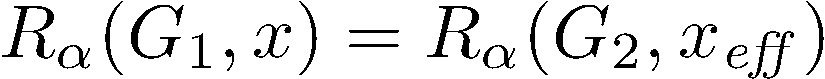
\includegraphics[width=0.4\paperwidth]{../Figures/RenormCaption}
\centerline{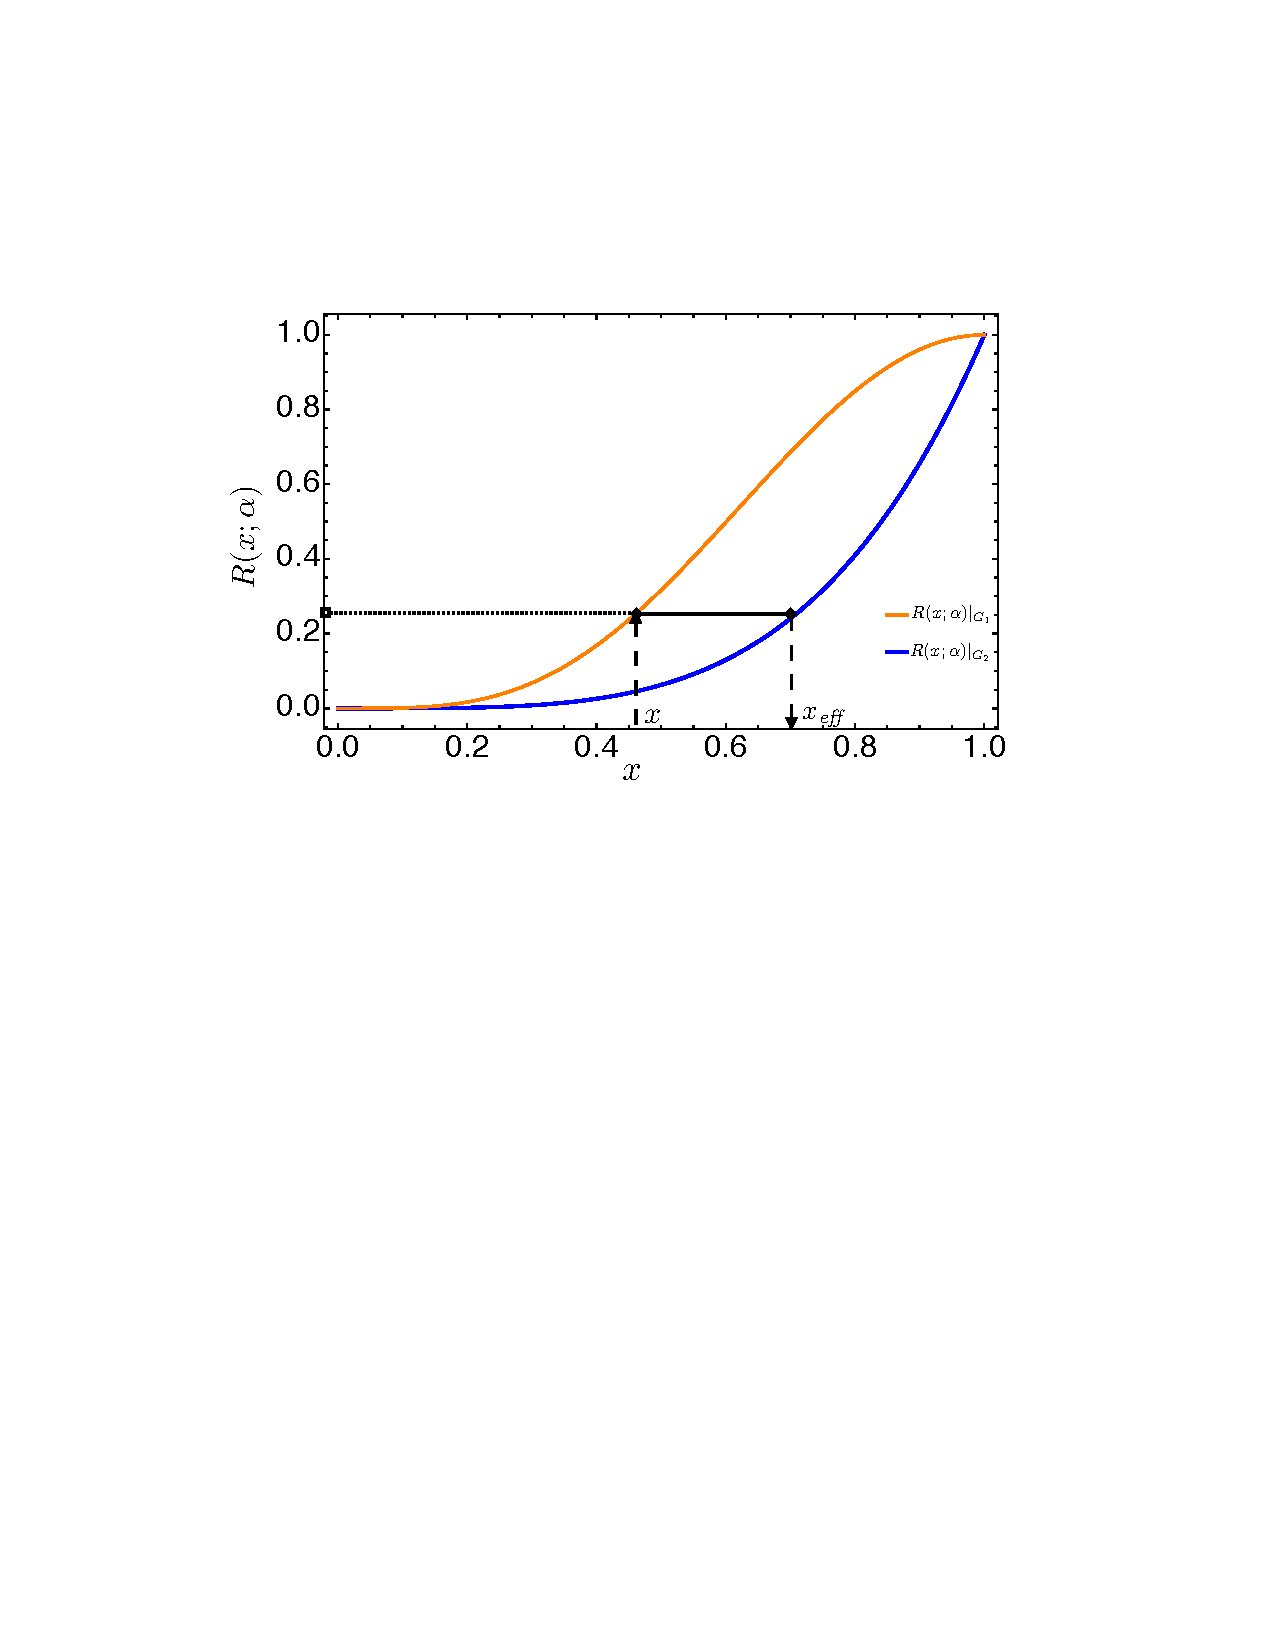
\includegraphics[width=0.90\paperwidth]{../Figures/Renorm}}

\vspace{-24pt}
\hyperlink{Applications}{\beamerreturnbutton{return}}
\end{frame}

%% ----------------------------------------------------------------------

\subsection{sensitivity analysis using Birnbaum importance}
\begin{frame}[label=CrossoverExample]
\frametitle{Ranking Edges: finding crossover in importance}

\centerline{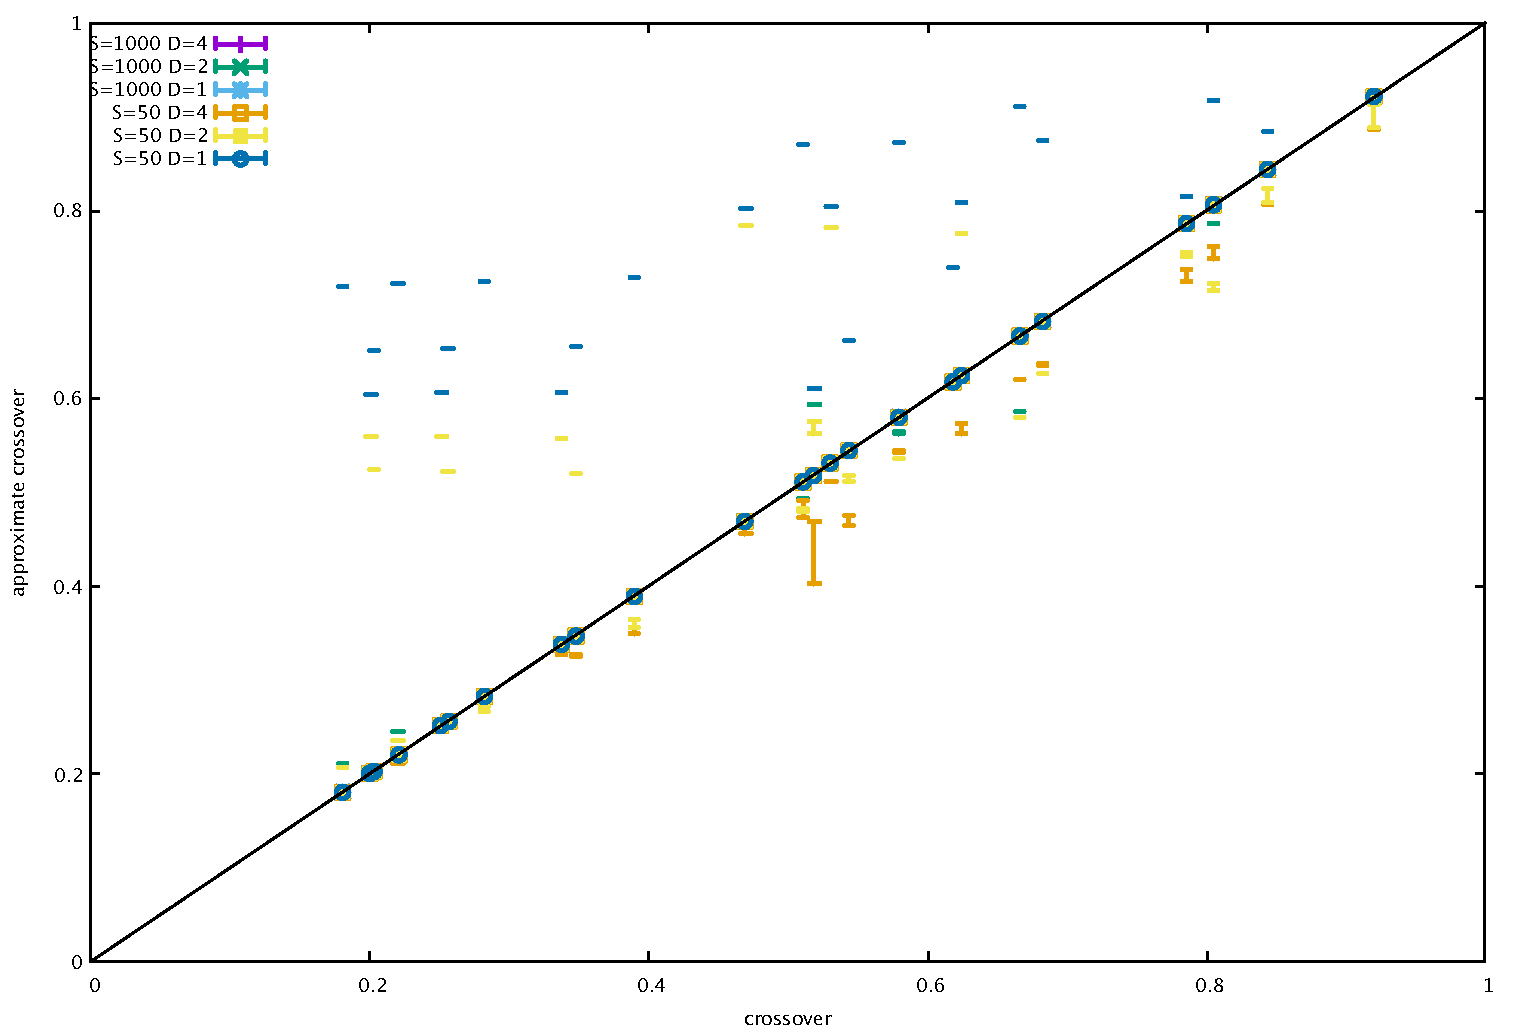
\includegraphics[height=0.90\textheight]{../Figures/crossover}}
\hyperlink{Applications}{\beamerreturnbutton{return}}
\hfil
\hyperlink{Crossover}{\beamergotobutton{What is crossover?}}
\end{frame}

%% ----------------------------------------------------------------------

\subsection{detecting communities using Birnbaum importance}
\begin{frame}[label=Community]
\frametitle{Detecting communities: finding planted partitions}
\centerline{
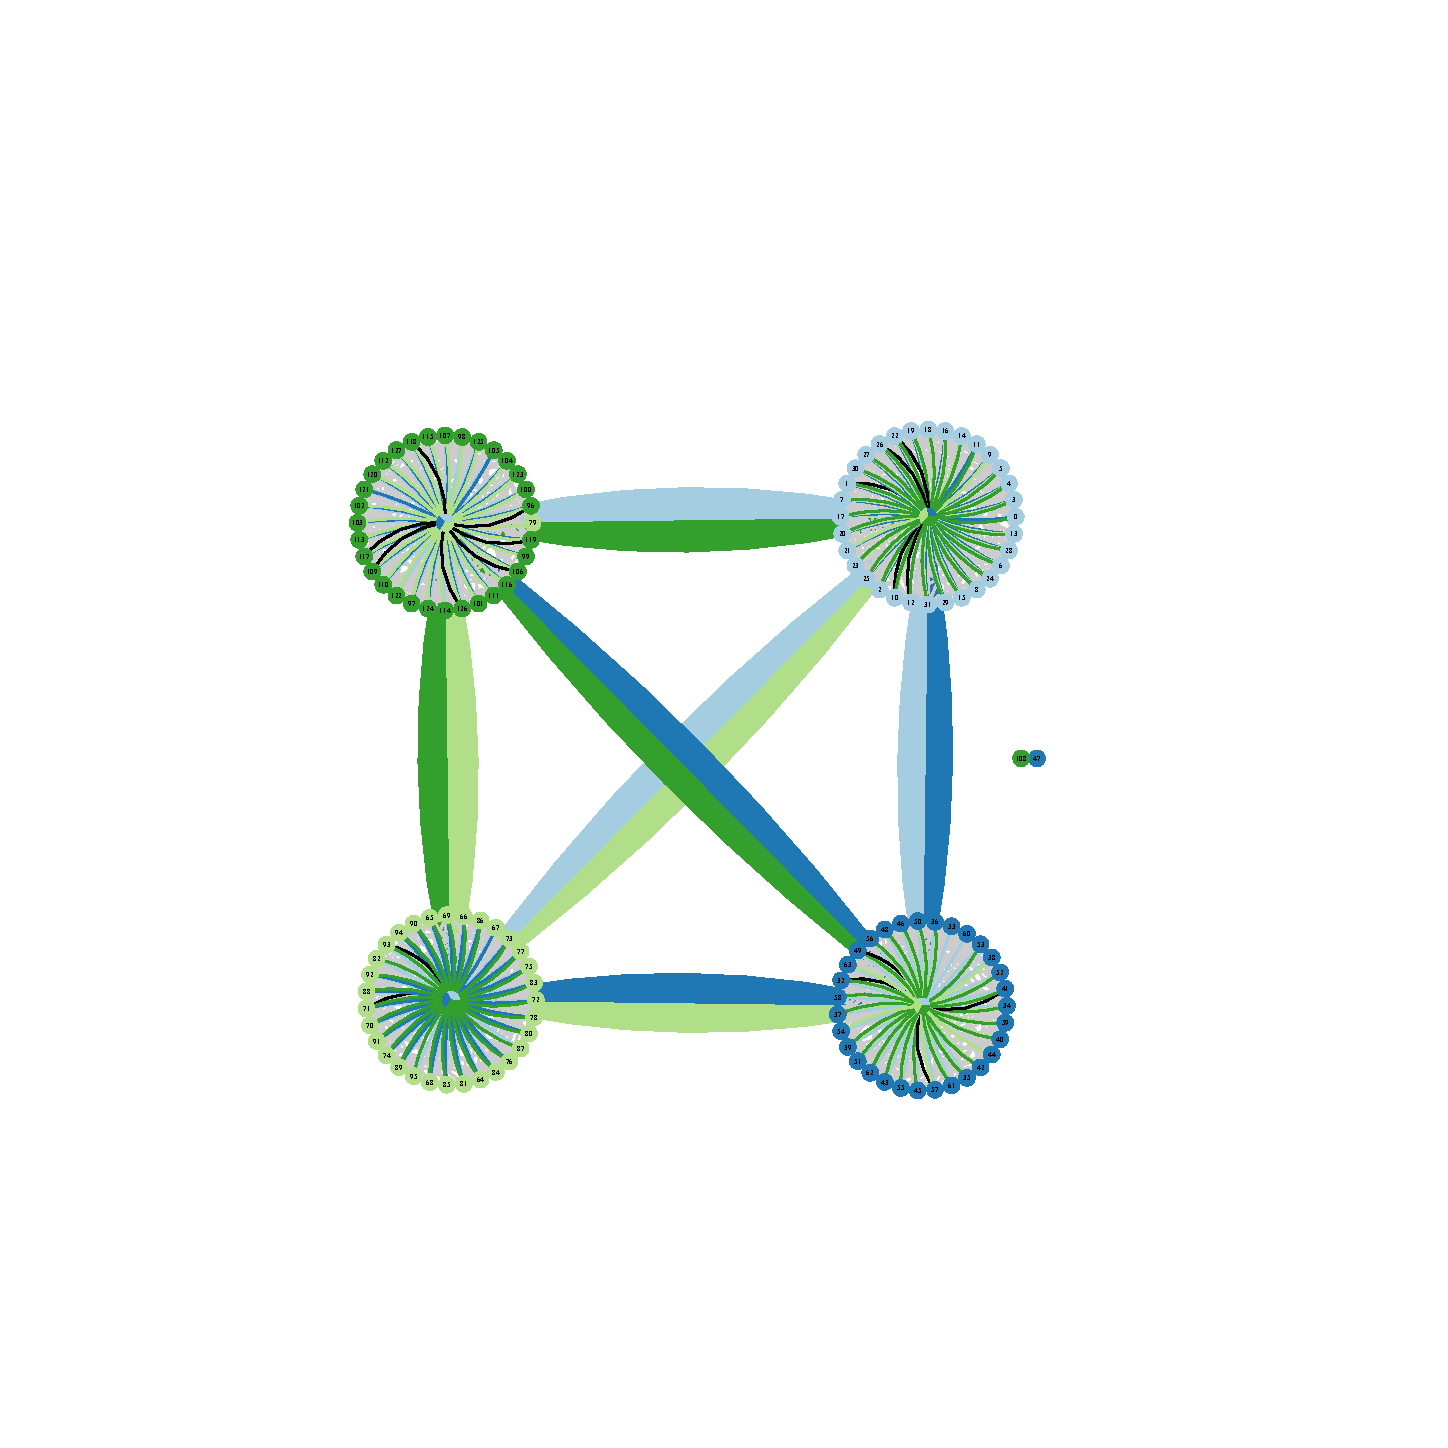
\includegraphics[height=0.75\paperheight]{../Figures/n100d3-07-eb-ecut}
}
\vspace{-0.025\paperheight}
\hyperlink{Applications}{\beamerreturnbutton{return}}
\hfil
\hyperlink{CommunityExpt}{\beamergotobutton{details of the experiment}}
\end{frame}

%% ----------------------------------------------------------------------

\subsection{graph reduction using Birnbaum importance}
\begin{frame}[label=GraphReduction]
\frametitle{Graph reduction}
\begin{remark}{Removing least important edges}
By iteratively removing the $k$ \alert{least} important edges, we can construct the subgraph of size $E-k$ whose reliability is closest to the original graph's.
Because of crossover effects, the reduced graph depends on dynamical parameters, e.g., $x$.
\end{remark}

\hyperlink{Applications}{\beamerreturnbutton{return}}
\end{frame}

%% ----------------------------------------------------------------------

\section{Applications}
\subsection{dual graphs}
\begin{frame}[label=GraphDuals]
\frametitle{Generating dual graphs}
\begin{example}{Dual}
The networks on the right are generated from those on the left by building a graph with a 1-1 correspondence between minimal struts in $G$ and minimal cuts in $G'$.
\end{example}

\centerline{
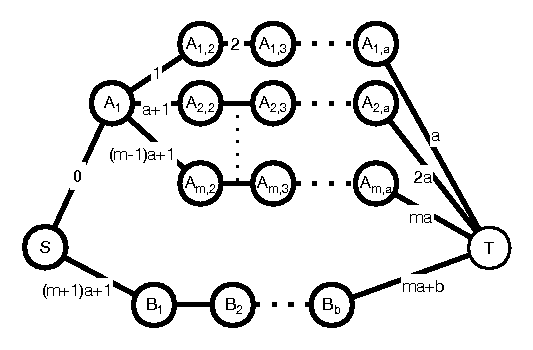
\includegraphics[width=0.45\paperwidth]{../Figures/toyMAB.pdf}
\raisebox{0.1\paperheight}{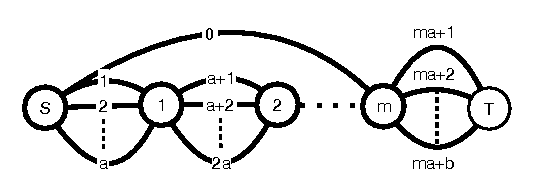
\includegraphics[width=0.45\paperwidth]{../Figures/toyMABdual.pdf}}
}
\vspace{-0.05\paperheight}
\begin{equation*}
%R_{G}(x) = x^b + x\left[1 - (1-x^a)^m\right]; \qquad 
R_{G'}(x) = 1 - R_{G}(1-x)
\end{equation*}

\hyperlink{Applications}{\beamerreturnbutton{return}}
\end{frame}

%%% ----------------------------------------------------------------------

\section{Cruxes:}
\subsection{estimation}
\begin{frame}[label=cruxes]
\frametitle{Finding cruxes}
\only<1-2>{\centerline{A lattice of the partially-ordered configurations}}
\only<3>{\centerline{Any path from top to bottom has one edge from a cut to a strut}}
\only<4-5>{\centerline{A simple search is guaranteed to lead to a minimal cut / strut}}
\only<1>{\centerline{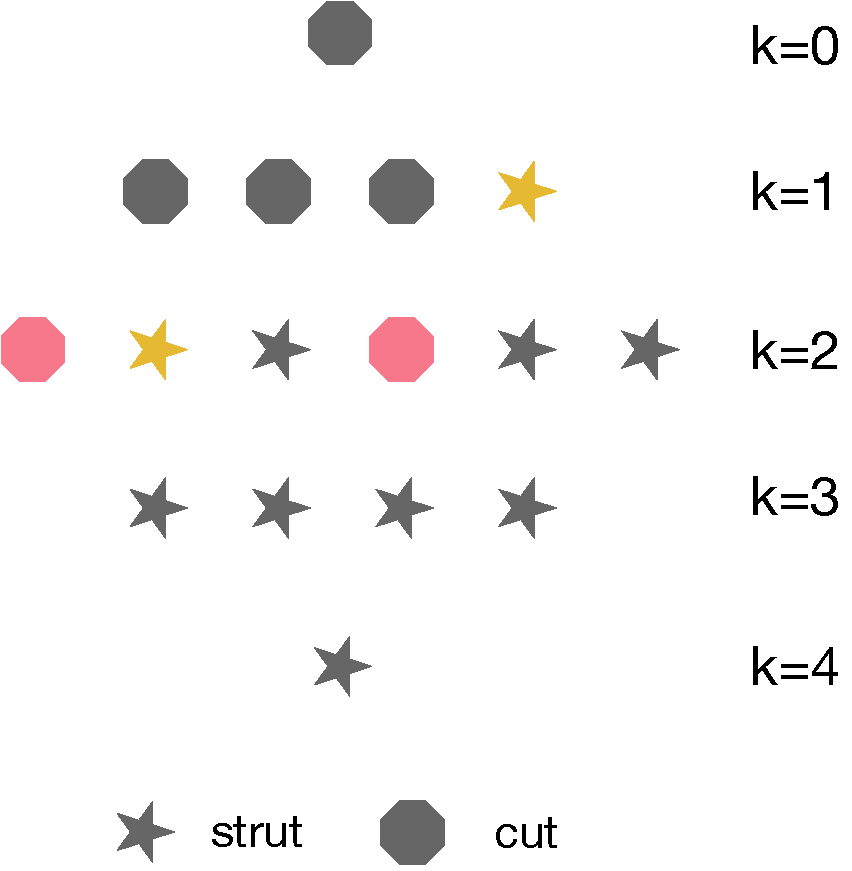
\includegraphics[width=0.5\paperwidth]{../Figures/CruxEdges1.pdf}}}
\only<2>{\centerline{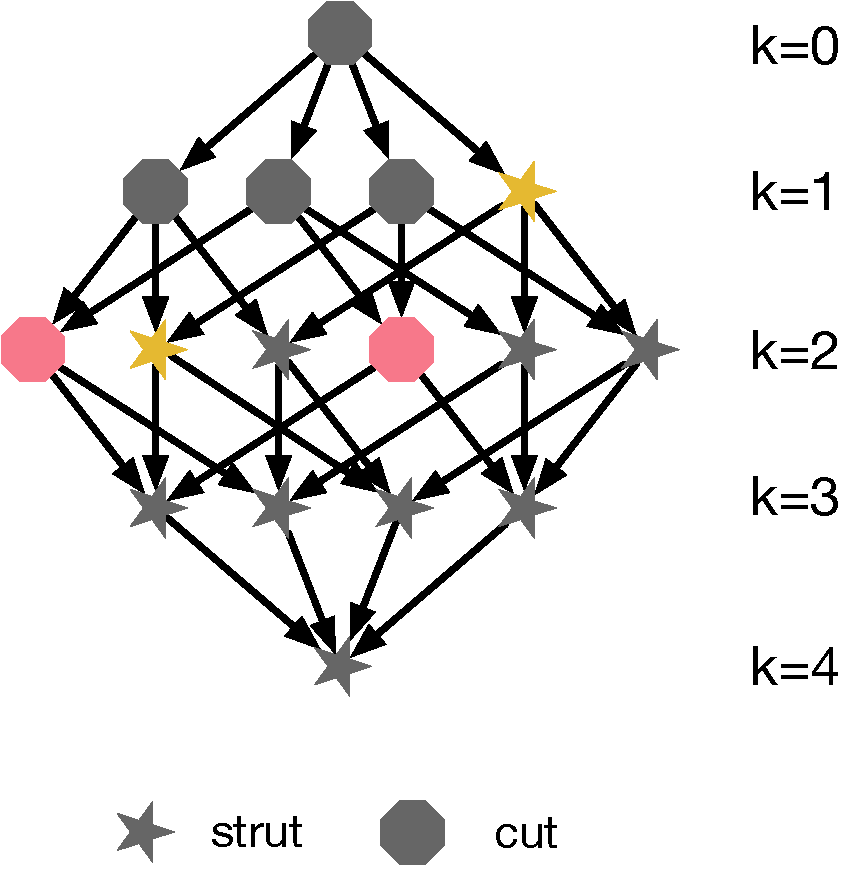
\includegraphics[width=0.5\paperwidth]{../Figures/CruxEdges1b.pdf}}}
\only<3>{\centerline{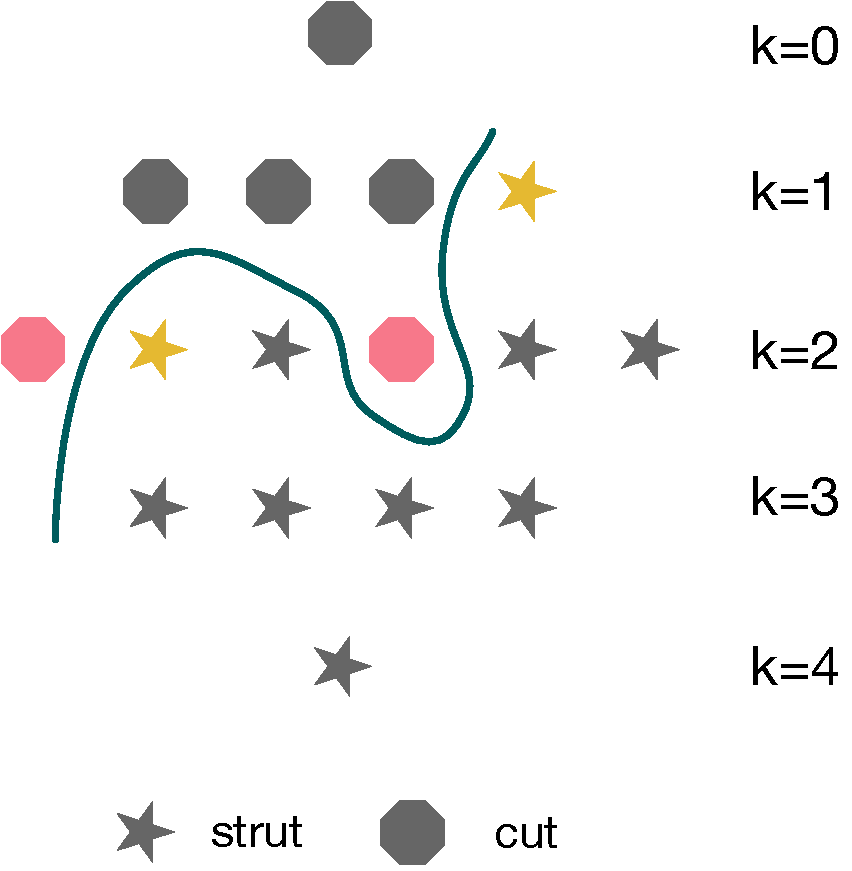
\includegraphics[width=0.5\paperwidth]{../Figures/CruxEdges2.pdf}}}
\only<4>{\centerline{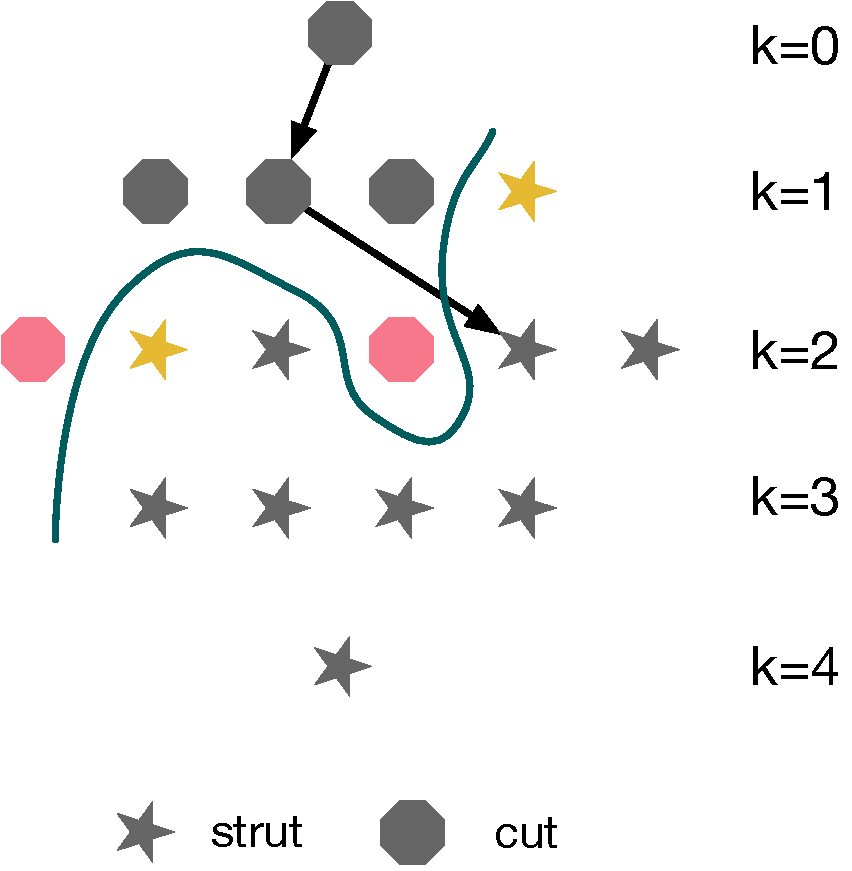
\includegraphics[width=0.5\paperwidth]{../Figures/CruxEdges3.pdf}}}
\only<5>{\centerline{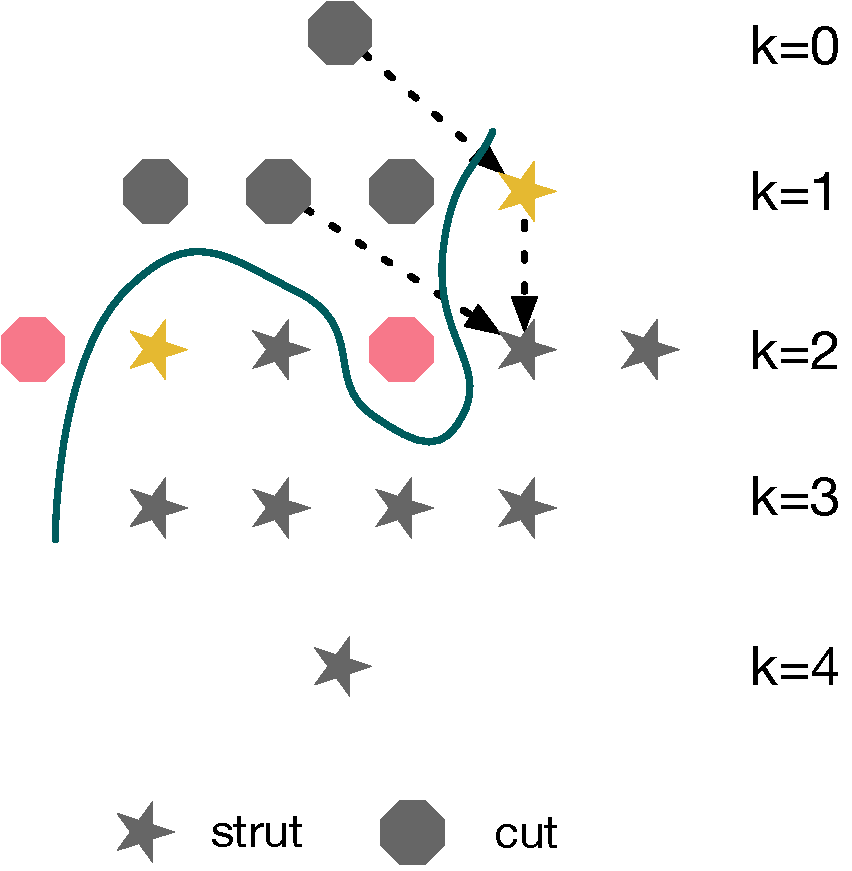
\includegraphics[width=0.5\paperwidth]{../Figures/CruxEdges4.pdf}}}
\hyperlink{monotonicity}{\beamerreturnbutton{return}}
\end{frame}

%% ----------------------------------------------------------------------

\section{Applications:}
\subsection{ranking edges using Birnbaum importance}
\begin{frame}[label=Crossover]
\frametitle{Crossover}

\begin{remark}{Crossover}
The relative contribution of different edges to the overall reliability -- the difference in their Birnbaum importance -- depends on dynamical parameters, e.g., $x$. It is possible for the relative ranks to switch at certain values of $x$.
For SIR dynamics on the family of toy networks, the ranks of the two most important edges switch when
$x^{b-1} = 1 - (1-x^{a-1})^m$.
\end{remark}

\hyperlink{CrossoverExample}{\beamerreturnbutton{return}}
\end{frame}

%% ----------------------------------------------------------------------

\begin{frame}[label=CommunityExpt]
\frametitle{A community detection experiment}
\begin{remark}{Community structure in a block stochastic\\
or ``planted $\ell$-partition'' graph}
We iteratively removed the highest-rank edge from a 128-node, 1024-edge graph in which we had planted 4 communities. The average degree of the nodes is 16, of which 9 are within its planted community and 7 are external. The algorithm finds  communities very similar to the planted ones across a wide range of parameters, and approximately 80\% of the edges it removes are among the 448 planted inter-community edges.
\end{remark}
\hyperlink{Community}{\beamerreturnbutton{return}}

\end{frame}

%% ----------------------------------------------------------------------

\section{Details:}
\subsection{Bezier interpolation (not to be confused with approximation!)}
\begin{frame}[label=Bezier]
\frametitle{Bezier polynomials for two-point Taylor interpolation} 
\vspace{-24pt}
$$
f(x) = \sum_{i=0}^N \alpha_i \textcolor{blue}{x^i} = \sum_{i=0}^N \overline{\alpha}_i \textcolor{blue}{(1-x)^i}; \quad
\hat{f}(x) = \sum_{k=0}^N \beta_k \textcolor{UVAOrange}{B(N,k,x)},
$$
where $B(N,k,x) \equiv {N \choose k} x^k (1-x)^{N-k} = B(N, N-k, 1-x)$.\\
\vspace{12pt}
Given $\{\alpha_0, \ldots, \alpha_m\}$ and $\{\overline{\alpha}_0, \ldots, \overline{\alpha}_{\overline{m}}\}$, find $\{\beta_0, \ldots, \beta_m\}$
and $\{\beta_{N-\overline{m}}, \ldots, \beta_N\}$ such that the first $m$ derivatives of $f$ and $\hat{f}$ match at $x=0$ and the first $\overline{m}$ derivatives of $f$ and $\hat{f}$ match at $x=1$.\\
 %This is a change of basis, accomplished by a lower-triangular matrix.
\vspace{12pt}
$\hat{f}$ is a kernel density estimator for $f$.\\
For large $N$, the change of basis automatically produces an analytic continuation for $f$.\\
\hyperlink{interpolation<2>}{\beamerreturnbutton{return}}
\end{frame}

%% ----------------------------------------------------------------------

\begin{frame}
\frametitle{Coming soon: a Mathematica demo illustrating interpolation}
\centerline{
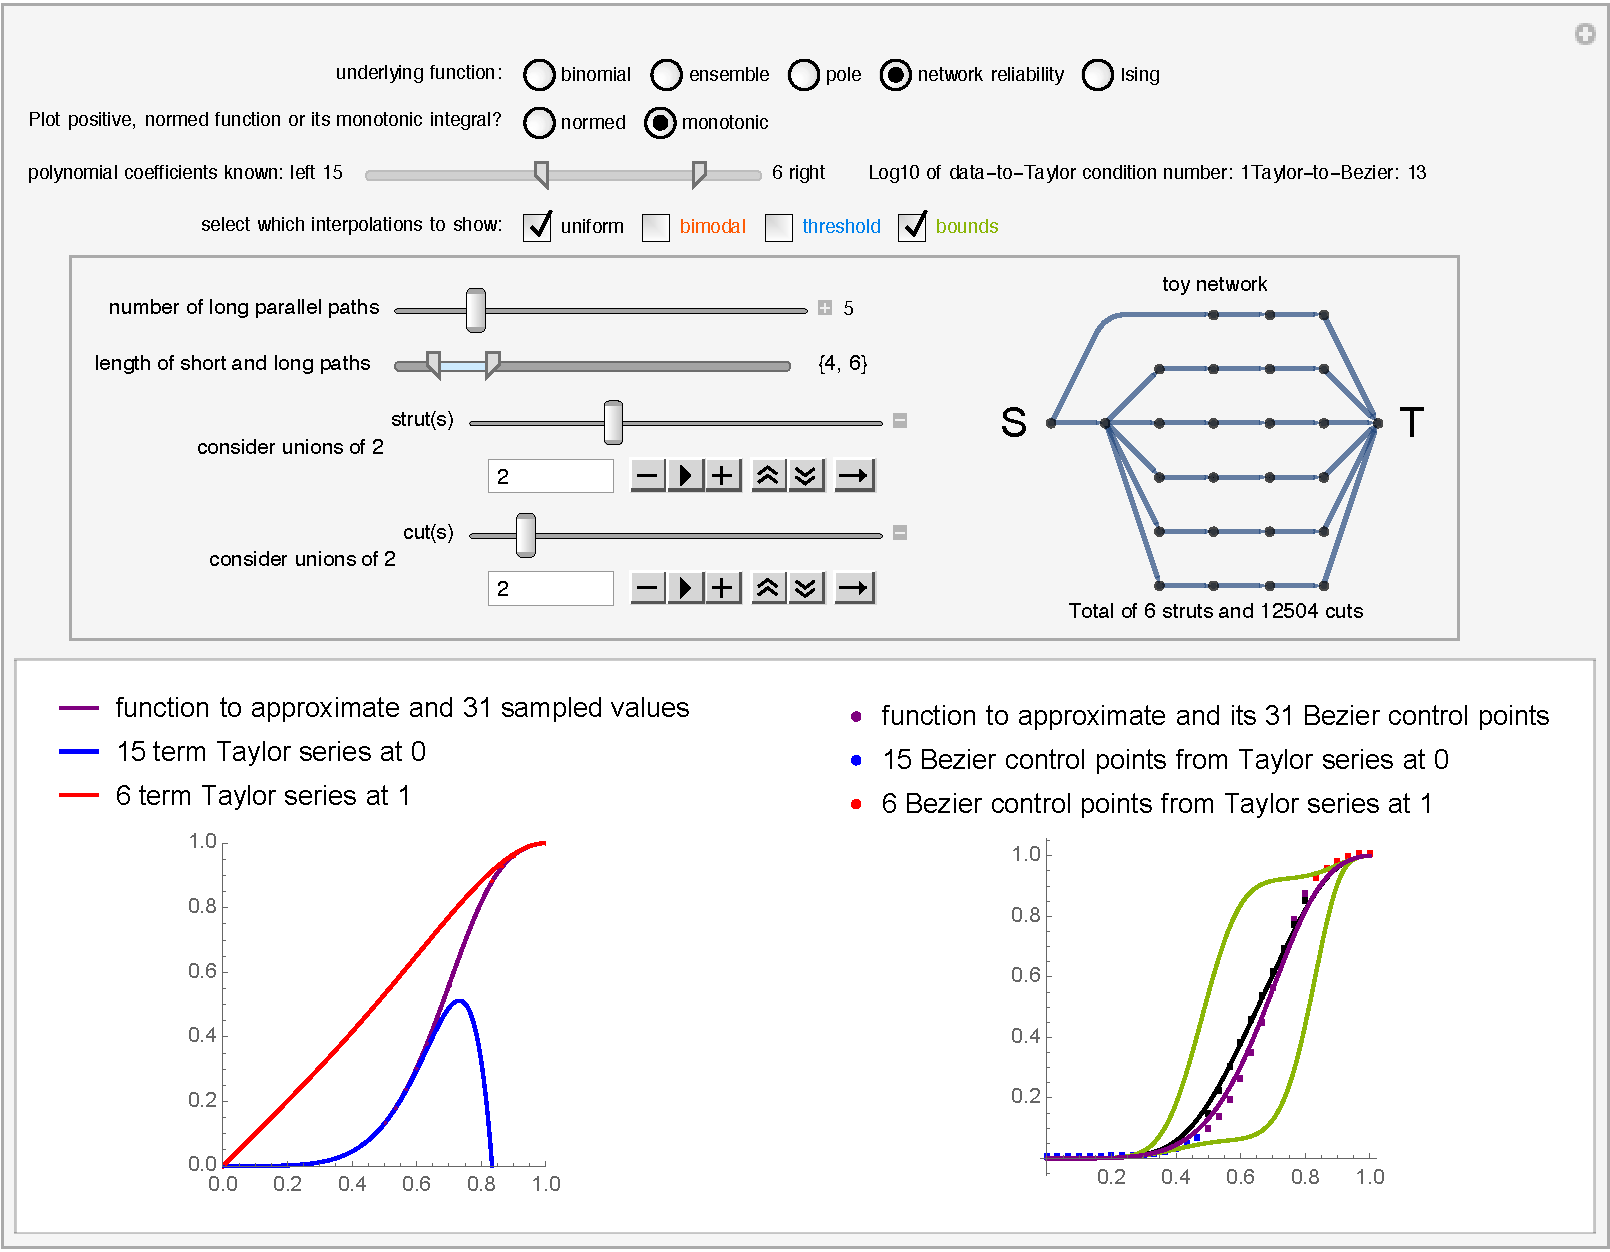
\includegraphics[height=0.7\paperheight]{../Figures/MathPage}
}
\hyperlink{interpolation<2>}{\beamerreturnbutton{return}}
\end{frame}

%%% ----------------------------------------------------------------------

\subsection{characterize network structure}
\begin{frame}[label=AddHealthDetails]
\small{
\frametitle{Details of the network comparison}
\begin{itemize}
\item AddHealth provides surveys of friendship networks in many schools.
\item Faux Magnolia is a network available in the statnet R package that reproduces several local properties of the friendship network for one of the schools in AddHealth.
\item The properties used to define reliability are that a fraction $\alpha$ of the population will be infected by a single, randomly selected infectious individual, for various $\alpha$'s.
\item The results indicate that the graph structures responsible for the difference involve roughly 70-80\% of the edges -- local statistics \alert{cannot} detect this difference.
\end{itemize}
}
\tiny{Add Health is a program project directed by Kathleen Mullan Harris and
designed by J. Richard Udry, Peter S. Bearman, and Kathleen Mullan Harris at the University of North Carolina at Chapel Hill, and funded by grant P01-HD31921 from the Eunice Kennedy Shriver National Institute of Child Health and Human Development, with cooperative funding from 23 other federal agencies and foundations. Special acknowledgment is due Ronald R. Rindfuss and Barbara Entwisle for assistance in the original design. Information on how to obtain the Add Health data files is available on the Add Health website (http://www.cpc.unc.edu/addhealth). No direct support was received from grant P01-HD31921 for this analysis.\\
Handcock, M. S., Hunter, D. R., Butts, C. T., Goodreau, S. M., Krivitsky, P. N., Morris, M., 2016. ERGM: fit, Simulate and Diagnose Exponential-Family Models for Networks. The Statnet Project (http://www.statnet.org). R package version 3.6.0.\\
}
\hyperlink{MCExample}{\beamerreturnbutton{return}}
\end{frame}

%% ----------------------------------------------------------------------

\againframe<4>{BinaryFunc}

\end{document}
